\vspace{-0.06in}
\section{Auction-SC Framework}
\label{sec:onlinealgo}
\vspace{-0.1in}
With a real-world SC system, the SC-Server will find out about a task and its properties only when it is released. The complexity of the many-to-many matching in addition to the need for immediacy (e.g., Uber) render the batch scheme impractical for real-world scenarios. Furthermore, in online monolithic-SC, scheduling multiple workers becomes the bottleneck and hence, real-time assignment is not guaranteed. For example, in New York City, during rush hours, there are as many as 10+ ride requests per second \cite{NYCTaxi}. Through experiments, we show neither the batched scheme nor the online monolithic-SC are able to process such throughput in real-time.

In this section we introduce Auction-SC which has neither shortcomings and generates real-time online assignments by splitting the matching and scheduling responsibilities between the server and the workers, respectively. This allows Auction-SC to scale up orders of magnitude higher than competing approaches. First we explain the auction framework and how tasks are dispatched to workers. Following, we discuss how workers compute and submit their bids and how the server assigns tasks to workers.
\vspace{-0.05in}
\subsection{Task Dispatching in Auction-SC}
\vspace{-0.05in}
Auction methods have been effectively used for assignment problems in dynamic multi-agent environments \cite{Mehta05}. The main advantage of auction methods are their simplicity and the fact that they allow for a decentralized implementation. Auction-SC considers workers as bidders and tasks as goods. Furthermore, the SC-Server plays the role of an auctioneer in Auction-SC. \cref{fig:dispatch} explains how tasks are dispatched to workers at a very high level: (1) Everything starts with a requester submitting a new spatial task to the SC-Server. (2) Once the SC-Server receives a new task, it notifies the available workers about the new task. (3) Each worker independently computes his bid by only considering the new task and his current schedule and submits a bid to the SC-Server. (4) Once all the bids are received, the SC-Server assigns the task to the worker with the optimal bid.

Broadcasting every incoming task to all available workers incurs a large communication cost on the system. Auction-SC lowers the communication cost by only sending an incoming task to the \textit{eligible workers} that are define as:
\vspace{-0.05in}
\begin{definition} [Eligible Worker]
\label{def:elig}
An available worker w is said to be eligible for performing a newly released task t, if and only if:
\vspace{-0.05in}
\begin{equation*}
distance(w, t) \leq w.d - t.r \wedge distance(w, t) \leq t.d - t.r
\vspace{-0.05in}
\end{equation*}
\end{definition}
\vspace{-0.05in}
\noindent This means an available worker \textit{w} is eligible for performing task \textit{t}, if it has enough time to reach the location of \textit{t} before either \textit{t} expires or \textit{w} leaves the system. Ideally, $distance(w, t)$ in \cref{def:elig} is equal to the road network distance between $w.l$ and $t.l$. However, computing the network distance for all workers is time consuming and hence, in Auction-SC, we use the Euclidean distance between $w.l$ and $t.l$ as a lower bound to their network distance. Furthermore, maintaining the exact location of every worker with a spatial index (e.g., R-Tree) while the workers' locations are constantly changing is too costly and cannot be done in real-time. Consequently, with Auction-SC, the SC-Server maintains a spatial grid on the location of the workers and only keeps track of the workers' cell. If we assume that worker $w$ is in cell $c_i$ of the spatial grid, then $distance(w, t)$ is computed as:
\vspace{-0.1in}
\begin{equation*}
distance(w, t) = distance(p^*, t) \ \mathrm{s.t.} \ p^* = \min_{p\ in\ c_i} \left\lbrace distance(p, t) \right\rbrace 
\vspace{-0.1in}
\end{equation*}

\noindent In other words, if any point in cell $c_i$ satisfies the constraints of \cref{def:elig}, all the workers in $c_i$ are considered as eligible workers. Therefore, upon arrival of a task $t$, the server first finds the cells that are within $t.d$ distance of the task (Shaded cells in \cref{fig:dispatch}) and broadcasts the new task only to workers within those cells.

\begin{figure}[h]
   \centering
    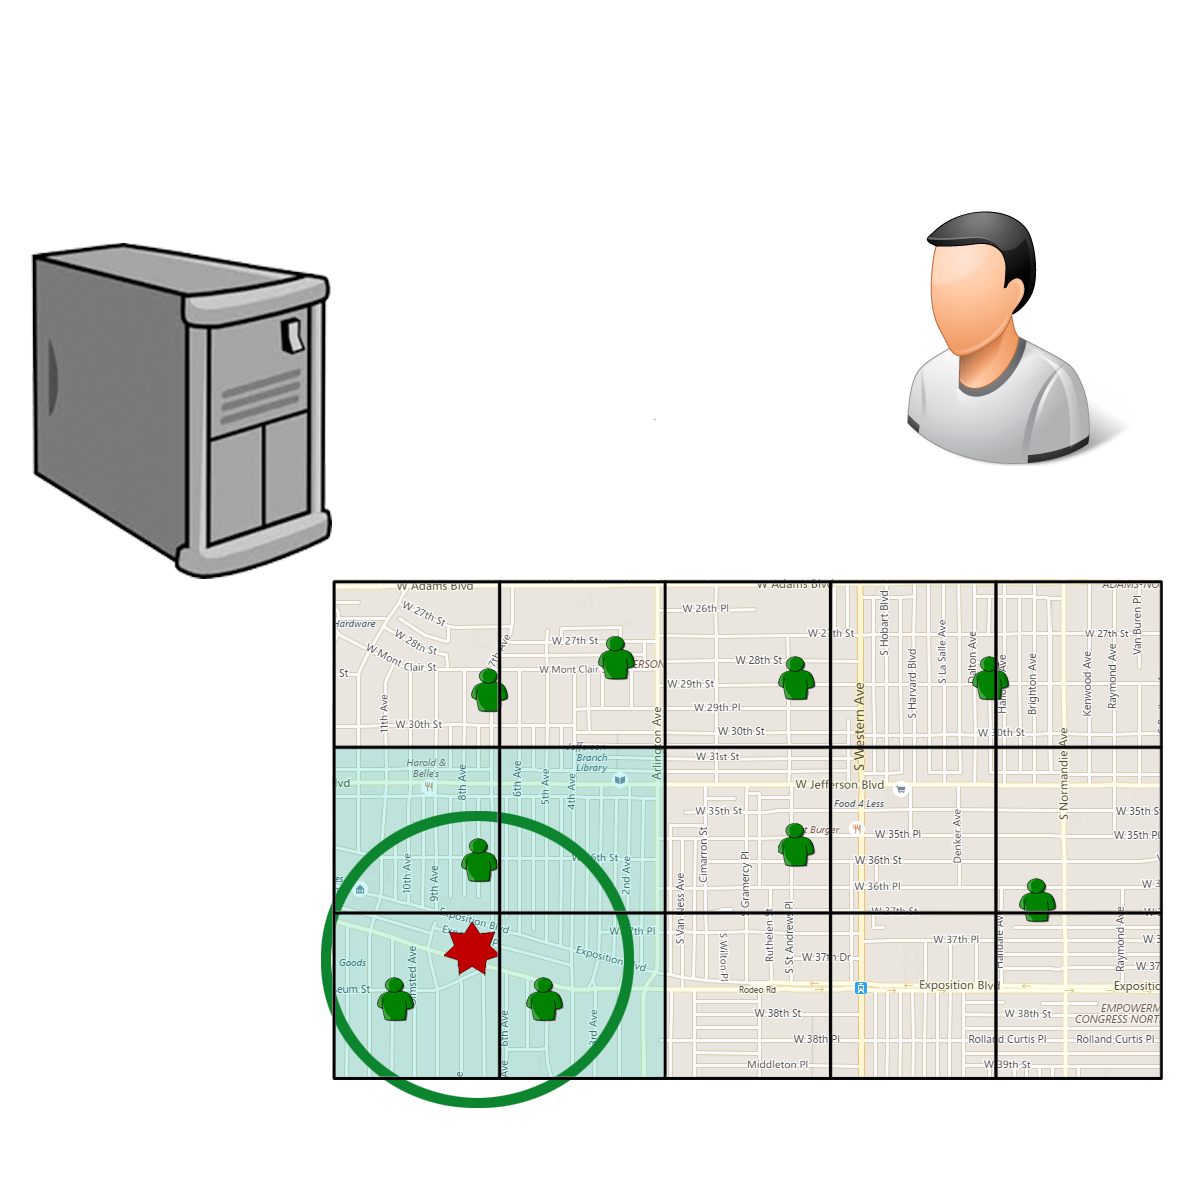
\includegraphics[width=0.75\columnwidth]{figures/scenario}
    \vspace{-0.15in}
    \caption{Task Dispatching in Auction-SC}
    \label{fig:dispatch}
\end{figure}

Once the eligible workers are notified about a new task, depending on the \textit{bidding heuristic}, which is common among all workers, each worker computes his own bid and submits the bid to the server. As mentioned earlier, the bid computation process is done by a software installed on the workers' cell phone. As a result, the process is the same for all workers and more importantly, it does not require any interaction with the human worker. The bidding process is performed similar to a \textit{sealed-bid auction} where workers simultaneously submit bids and no worker knows how much the other workers have bid. The SC-Server selects the worker with the optimal bid as the winner and matches the task with that worker.

\begin{algorithm}
\caption{OnlineTASC($W, t$)}
\label{algo:OnlineTASC}
\begin{algorithmic}[1]
\REQUIRE $W$ is the set of currently available workers and $t$ is a task that has just released
\ENSURE Either $w \in W$ as the worker task $t$ should be assigned to or \emph{null} if no worker is selected
\STATE $w_{selected} = $ \emph{null}
\STATE $Bids = \emptyset$
\STATE Broadcast $t$ to every $w \in W_t$ \label{line:broadcast}
\WHILE {$w \in W_t$ has not submitted bid}\label{line:while_start}
	\STATE $Bids \leftarrow \left\langle w, bid \right\rangle$ \label{line:rec_bid}
\ENDWHILE \label{line:while_end}
\STATE $w_{selected} = $ SelectBestBid$(Bids)$ \label{line:select}
\RETURN $w_{selected}$
\end{algorithmic}
\end{algorithm}

\cref{algo:OnlineTASC} outlines the process of assigning an incoming task $t$. $W_t$ in line~\ref{line:broadcast} is the set of eligible workers for task \textit{t}. While there are workers who have not submitted their bids yet (lines~\ref{line:while_start}-\ref{line:while_end}), the server will keep accepting bids and adds every received bid to the set $Bids$ (line~\ref{line:rec_bid}). Once all eligible workers submit their bids, the \emph{SelectBestBid()} method (line~\ref{line:select}) returns the worker with the optimal bid. In case of a tie, the \emph{SelectBestBid()} method, randomly selects one worker among the ones with the optimal bid.

We end this section with a brief discussion on the communication cost in Auction-SC. As a result of task dispatching and bid submission in Auctions-SC, it seems that the communication cost in this framework will limit its advantages over existing approaches: i.e., batched assignment and monolithic-SC. However, regardless of the approach, there is always going to be some communication cost. In both the batched and online monolithic-SC approaches, the SC-Server is responsible for performing scheduling. To perform scheduling, the server requires the \textit{exact} location of the workers, which means the workers have to constantly communicate with the server to update their locations. At the very least, each time a new task arrives, the server needs to communicate with the eligible workers to get their exact locations. On the other hand, the server in Auction-SC does not require the exact location of the workers as it is not responsible for performing scheduling for the workers. Instead, the server in Auction-SC has some communication cost for dispatching tasks and submitting bids. Nevertheless, in our experiments, we do consider the communication cost in Auction-SC and since other approaches do not discuss their communication model, we ignore the communication cost in other approaches. We still show that Auction-SC scales better than both the batched and the online monolithic-SC approaches.

\vspace{-0.05in}
\subsection{Worker's Bid Computation}
\label{subsec:bidding}
\vspace{-0.025in}

With Auction-SC, every worker computes his bid using a predefined bidding rule. A worker's bid represents how good it is for him to be matched with the task. When computing a bid for a task, the workers have no knowledge about other tasks that might arrive in the future. Consequently, they have to make a greedy decision based on their current status. Existing studies have used various heuristics in order to match tasks with workers; e.g., spatial region \cite{Cheng16}, nearest neighbor \cite{Fonteles15,Kazemi12,Guo16} and earliest expiring task \cite{Fonteles15}. All these heuristics are applied to an SOM approach where the schedule of the worker is ignored. In this section we introduce a new heuristic where a task is assigned to a worker who can insert it into its schedule better than other worker and hence, it is called \emph{Best Insertion (BI)}.

Intuitively, if a worker spends less time to complete a task, it will likely have more time for performing other tasks. In BI, the server gives priority to workers that can better insert the incoming task into their schedules. Auction-SC considers the \textit{extra time} each worker will need to complete the new task in addition to its current schedule. The first step in computing a bid, is for each worker to find the best schedule which consists of all the uncompleted tasks that have already been assigned to the worker, in addition to the newly incoming task. For this, each worker runs \cref{algo:can_schedule} locally to find such schedule.

\begin{algorithm}[!ht]
	\caption{FindBestSchedule($f, r, bt, bs, start$)}
	\label{algo:can_schedule}
	\begin{algorithmic}[1]
		\REQUIRE \emph{f} and \emph{r} are lists of tasks that have been added and need to be added to a valid schedule, respectively. \emph{bt} and \emph{bs} are the best finish time and corresponding schedule observed so far and \emph{start} is the current time.
		\ENSURE $bt, bs$ as the best finish time and corresponding schedule for input points if a valid schedule exists. Otherwise $\infty, \emptyset$
		\FOR{$t$ \textbf{in} $r$}
			\STATE $f' = f$
			\STATE $f'$.add($t$)
			\STATE $t =$ GetFinishTime($f', start$)
			\IF{$t \neq \infty$}
				\STATE $r' = r$
				\STATE $r'$.remove($t$)
				\IF{$r'$.size $== 0$}
					\RETURN $t, f'$
				\ENDIF
				\STATE $t, s =$ FindBestSchedule($f', r', bt, bs, start$)
				\IF{$t < bt$}
					\STATE $bs = s$
					\STATE $bt = t$
				\ENDIF
			\ENDIF
		\ENDFOR
		\RETURN $bt, bs$
	\end{algorithmic} \vspace{-1mm}
\end{algorithm}

\cref{algo:can_schedule} utilizes a branch and bound method to search all possible orders of its uncompleted tasks in addition to the new task. The idea is to enumerate every valid schedule, calculate its finish time and choose the one with the earliest finish time. Therefore, the algorithm recursively performs an exhaustive search to find the best valid schedule. Given the set of tasks that have already been added to the schedule (i.e., set $f$), and the remaining tasks (i.e., set $r$), at each iteration of \cref{algo:can_schedule} (lines 1-17), one task from $r$ is added to $f$ (lines 2-3). Each time a new task is added to $f$, the algorithm checks whether this partial schedule is valid. If the partial schedule is invalid, \textit{GetFinishTime} in line 4 returns $\infty$ and the search continues to the next branch. Otherwise, the variable $t$ contains the finish time of the partial schedule $f$. If the remaining tasks set , $r$, gets empty, the search on the current branch stops and the current branch's finish time and corresponding schedule is returned (lines 8-9); otherwise, it recursively checks the new branch $r'$ (line 11). The best finish time is updated once the search finds a finish time $t$ smaller than the best finish time seen so far $bt$ (lines 12-15).

Figure~\ref{fig:bAndb} shows an example of using \cref{algo:can_schedule} to find the best schedule with three tasks. Each rectangle represents a node in the search tree, where the left and right sections contain the scheduled and the remaining tasks, respectively (sets $f$ and $r$ in \cref{algo:can_schedule}). Initially the set $r$ is started with all three tasks. The shaded rectangles contain an invalid partial schedule in the left section and hence, the tree does not expand below them. The search continues until all the branches have been visited and the complete schedule with the smallest finish time is returned.

\begin{figure}[!ht]
	\centering
	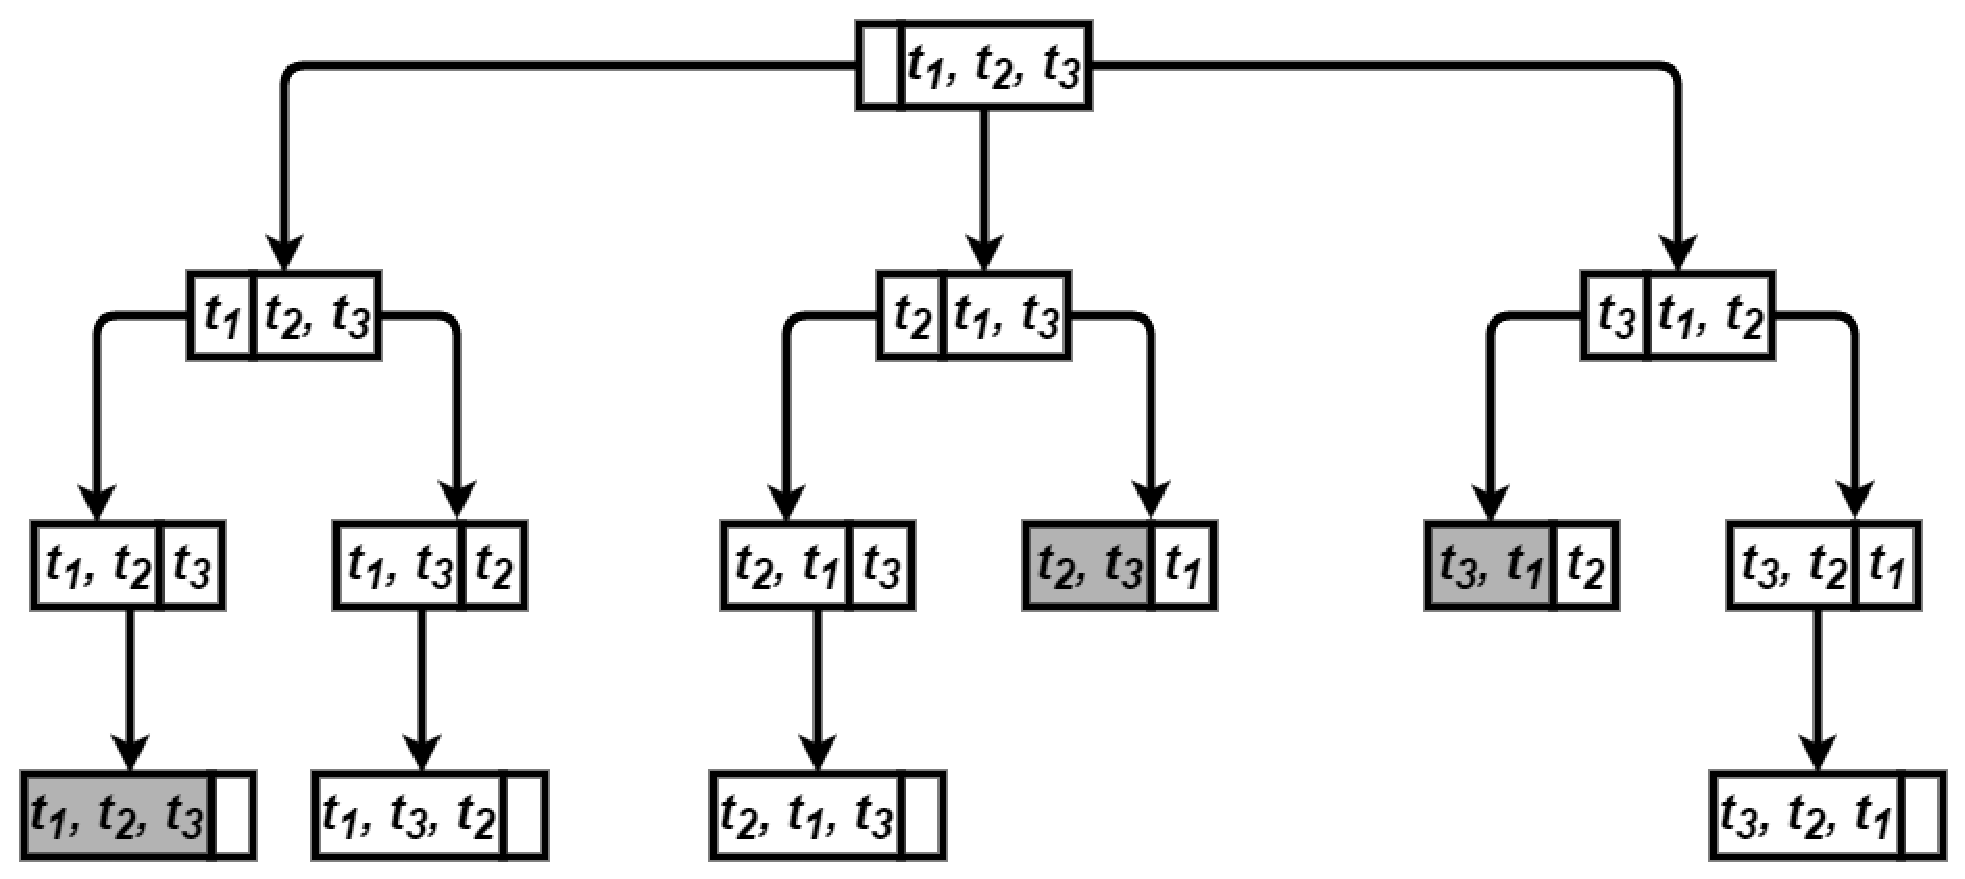
\includegraphics[width=0.75\columnwidth]{figures/bAndb}
	\vspace{-0mm}\caption{Illustration of \cref{algo:can_schedule}} \vspace{-2mm} \label{fig:bAndb}
\end{figure}\vspace{-0mm}

Running an exhaustive search for large number of tasks can be time consuming. However, in our experiments on both real world and synthetic data, we realized that the number of uncompleted tasks at each point of time for each worker, remains in a range where even the exhaustive search can be done in real-time for a single worker. The reason is that, as time passes and new tasks arrive, the worker also completes older tasks and removes them from its schedule. In cases where running \cref{algo:can_schedulue} takes too long, we can replace this computation with an approximate algorithm (e.g., the Nearest Insertion algorithm \cite{Rosenkrantz74}). In our experiments, we show that running an approximate algorithm for the scheduling phase, reduces the  the assignment rate (i.e., the percentage of tasks that get completed) by less than 5\%.

At each point in time, every worker has a schedule and knows the finish time of his schedule (i.e., $f_{current}$). If the schedule of a worker is empty, then $f_{current} = \mathnormal{current \ time}$. After running \cref{algo:can_schedule} and finding the potential optimal schedule that adds a new incoming task to the worker's current schedule, each worker can compute the finish time of this potential schedule as well (i.e., $f_{potential}$). Knowing both $f_{current}$ and $f_{potential}$, each worker can compute the difference between the two times as the \emph{extra time} he requires to be able to finish all his tasks if the new incoming task is assigned to it. Using the BI heuristic, each worker $w$ submits his bid to the server as: $ bid_w = f_{potential} - f_{current}$. The smaller the the difference between $f_{current}$ and $f_{potential}$, the better the worker can fit the new task in his schedule. Therefore, once the server receives the bids of every worker, it will assign the task to the worker with the smallest bid.